\chapter{Sample Chapter}
\label{ch:sample_chapter}

This is a generic chapter with code on how to add figures, quotes, code snippets etc.

\begin{quote}
Oh look, quoted text! Such magical.
\begin{enumerate}
\item There is even a list inside the quote!
\item Science has come so far.
\end{enumerate}
\end{quote}

Aha a figure.

%[H] forces LaTeX to place the figure HERE, overriding all defaults.
%[h] asks LaTeX nicely to place the figure HERE if possible, no forcing.
%leaving it empty means you trust LaTeX to place the figures however it deems correct.
\begin{figure}[H]
\centering
\captionsetup{justification=centering}

\includegraphics[width=8cm]{\dir/plots/buzo.JPG}
\caption{Best dog in the world.}
\label{fig:buzo}
\end{figure}

Here's how to add a code snippet. Put the file in the "code" folder in this chapter's directory and direct the path to it. Also set the language and caption as you need.

\begin{figure}[H]
\lstinputlisting[language=Python,caption=Sample pseudocode.]{\dir/code/sample.py}
\label{listing:sample_listing}
\end{figure}

And now here's how to add a piece of code in-line, by typing it out in the \TeX file itself.
\begin{figure}[H]
\begin{lstlisting}
sample = [10,5,2,3,6]
print(sample)
\end{lstlisting}
\end{figure}

And now a table!

\begin{figure}
\centering
\begin{subfigure}{\textwidth}
  \centering
  \begin{tabular}{ | c c |}
    \hline
    Number of interactions & Number of pairs\\ \hline
    1 & 1787 \\ 
    2 & 694 \\
    3 & 442 \\
    42 & 13 \\ 
    100 & 1 \\ 
    1983 & 1 \\
    \hline
    Maximum number of interactions & 2949 (1 pair) \\
    Mean number of interactions & 32.40 \\
    Median number of interactions & 3 \\
    \hline
  \end{tabular}
\caption{Statistics on the degree of edges.}
\label{table:degree_of_edges}
\end{subfigure}%

\begin{subfigure}{\textwidth}
\centering
\captionsetup{justification=centering}
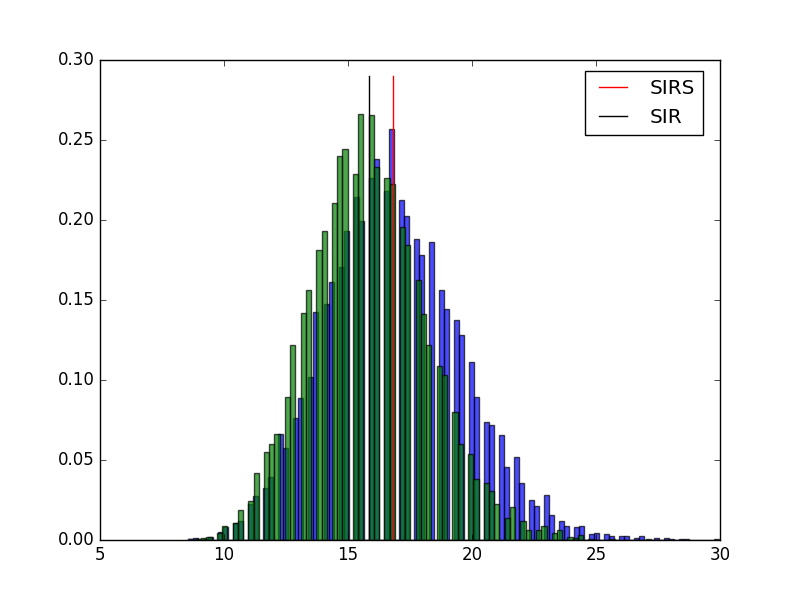
\includegraphics[width=10cm]{\dir/plots/sir_vs_sirs.png}
\caption{Some shit.}
\label{fig:some_shit}
\end{subfigure}
\caption{The distribution follows a heavy-tailed power law as seen in \ref{fig:degree_of_edges_hist} inset.}
\end{figure}

Notice how the table and the figure are added as "sub-figures". You can use this code to add two images side by side.

And while writing the thesis if there's something you want to come back to later, just add a highlighted comment like this. \hlc[pink]{Citation Needed}

This is how you refer to different labels in your document. \hyperref[ch:appendix]{Appendix} and \hyperref[ch:background]{Background}.

You might also want to add citations. Add your citations to the "bib" file then add them to the text using the \lstinline|\Cite| command (looks like this \Cite{mastrandrea2015contact}) or \lstinline|\Citeauthor| command (looks like this \Citeauthor{rosvall2014memory}. For your citations to actually work you first need to compile your \TeX file using PDFLaTeX, then by BibTeX and then by PDFLaTeX again.